\documentclass[a4paper]{article}

%% Language and font encodings
\usepackage[english]{babel}
\usepackage[utf8x]{inputenc}
\usepackage[T1]{fontenc}

%% Sets page size and margins
\usepackage[a4paper,top=3cm,bottom=2cm,left=3cm,right=3cm,marginparwidth=1.75cm]{geometry}

%% Useful packages
\usepackage{amsmath}
\usepackage{amssymb}
\usepackage{graphicx}
\usepackage[colorinlistoftodos]{todonotes}
\usepackage[colorlinks=true, allcolors=blue]{hyperref}
\usepackage{url}
\usepackage{listings}
\PassOptionsToPackage{hyphens}{url} 

%\setlength{\parindent}{0pt}%
% replaced by
\usepackage{parskip}


\title{Sampling Based Motion Planning Algorithms}
\author{299r Fall 2017 by Nao Ouyang}

\begin{document}
\maketitle

\begin{abstract} 
This paper covers the work I did for my research rotation with Professor Lucas
Janson in Fall of 2017. The rotation focused around sampling-based motion
planning algorithms which are frequently used in robotics (my area of
interest).  The rotation can be roughly divided into three main components: 1.
Understanding the algorithms 2. Understanding the proofs of the algorithmic
properties 3. Computer simulations of the algorithms. The specific algorithms
covered include: 1. RRT and it's optimal variant, RRT* 2. PRM and it's
simplified variant, sPRM 3. FMT* Finally, I'll write a section reflecting on my
experiences this semester.

\end{abstract}

\section{Introduction}

The goal of sampling-based algorithms is to reduce high-dimensionality
problems, which in practicality cannot be solved exactly, to something
manageable by sampling randomly within the space to find paths.

The two foundational algorithms are Rapidly Exploring Random Trees, aka RRT;
and Probabilistic Roadmaps, aka PRM. The first is used for on-line path
planning, as it rapidly converges to a feasible path with increasing number of
samples. On the other hand, probabilistic roadmaps make a graph covering the
space. This graph can be reused for multiple start and goal locations, whereas
the RRT algorithm generates a path for a specific pair of start and end points.

Generally proofs cover the feasibility, optimality, and computational complexity
of the different algorithms. Researchers seek to charaterize properities that
help determine how many samples might be required to cover a space well enough
to have a high probability of finding a feasible path (if it exists), including
in terms of how fast this probability changes as (for instance) a function of
the number of samples.

Although here we will present 2D (xy) examples of the algorithms where the robot
is a point, these algorithms can be applied to any dimensions. For instance, we
can imagine the dimensions for a multirotor might include x,y,z and also roll,
pitch, and yaw of the copter. However, as the number of dimensions we must sample in
increases, we encounter what is called the "curse of dimensionality". In many of
the proofs, one will encounter a $^{1/dim}$ exponent where, for instance, the
convergence of a solution will slow down drastically the number of dimensions
increases.

\subsection{How people represent these problems}

In all of these algorithms, we have a perfect map of the environment and can
check for node and edge collsions. Addititionally, we have a goal region rather
than a point goal, as the probability of sampling exactly the goal node is
essentially zero.

!! TODO: go over standard problem formuation, e.g. $X_{free}$, $B(\mu, r)$, etc. %TODO 

\section{Algorithms}

Both PRM and RRT algorithms are straightforward, requiring less than 10
lines of pseudocode each \footnote{Psuedocode as written in that "algorithm"
format all CS papers seem to use, with the $\gets$ signs.} 

The pseudocode for the algorithms may be found in \cite{RRT*}. Here I will
attempt a more casual description. 


!! TODO: go over all the symbols used e.g. set notation %TODO 

\subsection{PRM}

We have two variables we control: the number of samples we use, which is
pre-determined, and also the connection radius. In later cases we will write
this connection radius as a function of the number of samples used in a
given run. 

The general idea of PRM is to sample uniformly over the free space (generally,
we actually *close* to uniformly by sampling over the entire space, collision
checking, and throwing out colliding nodes). We then have a "local planner"
which connects each point to its neighbors. Two commonly used methods are
"k-nearest", in which points are connected to its k nearest neighbors; and
otherwise by a distance threshold. (for the purposes of this report, we will
work in metric space, where the triangle inequality holds, and use Euclidean
distance as the distance metric). If we sample enough points, according to percolation
theory, we will end up with a well-connected graph (as opposed to isolated
clusters).

Finally, when given a specific set of start and end points, we can use any
standard graph search algorithm, such as A*, to find a path in the graph between
the start and end points.

Simplified PRM, or sPRM, differs only in that connections between vertices in
already connected components are allowed. This makes the implementation easier.
In the original PRM, these connections were avoided as they do not contribute as
much to the connectivity of the graph.

\subsection{RRT}

In RRT, we build a tree instead of a graph. This tree grows from the start node
and terminates when it connects to the goal node. Whereas in PRM where we sample
all the points at once and then run a local planner and finally a graph search,
in RRT we teratively randomly sample a point in space. In this way RRT is more
suitable for online applications, where we care more about finding a solution
fast than have a good coverage of the entire space.

We first include the starting point in the tree. Then, we randomly sample a
point in free space, and then connect it to the nearest node in the tree. If the
neighbor is outside the connection radius, then we "steer" (or take a step of
distance $r$ from the neighbor to the sample), and add that closer node to the tree
(instead of the original sampled point). Of course, the edge we add must be
collision free. 

Of note, randomly sampling in the entire space is preferable to, for instance,
sampling random control inputs from the existing tree. In the latter case, new
points will tend to cluster around existing points. With sampling across all of
free space, points will tend to land in unexplored space (since the unexplored
space will be of greater area than the explored space, thus the probability of
sampling in unexplored space is bigger). Voronoi diagrams can help visaulize
this effect of random sampling. 

!! Todo: add picture of voronoi diagrams %TODO

\subsection{PRM*}

In order to guarantee that PRM will be asymptotically optimal, we simply define
a lower limit on the connection radius as a function of the number of samples.

\subsection{RRT*}

An unfortunate downside of RRT is that, because it stops growing the tree as
soon as it reaches the goal node, it is likely to return a suboptimal route. In
fact, it can be proven that as $\lim_{n\to \infty}$, RRT is \textbf{guaranteed} to return a suboptimal path. 

In order to guarantee that RRT will return an optimal path as $\lim_{n\to
\infty}$, we must introduce a "rewire" function. For each point we put down, we
will rewire it and its neighbors to make sure that the each point in the tree is
reached with least cost (all paths are "shortest paths"). Rewiring involves
removing an edge and replacing it with another edge. Additionally, as the number
of nodes we have sampled increases, we decrease the connection radius (as a
function of n).

This rewiring step is done for two conditions.

Specifically, when we add a node, we check that the edge to its nearest neighbor
in the tree is collision-free (that is, we check that the node can be added to
the tree at all). After that, we consider the edges to all points within a
radius of the new point. If one of edges results in a lower path cost (where
path cost is defined starting from the origin) than the edge we just created, we
erase the first edge and add in the latter. 

After that, we try all the edges to neighbors in distance r from the new point,
and if that new path to the neighboring edge results in a smaller cost than the
current path to the neighboring edge (from the origin), then we deleted the
parent and add in the edge connecting $x_new$ to the neighbor.

!! Todo: image of example of rewiring step's two cases %TODO

\subsection{FMT* (Fast Marching Tree)}

\subsubsection{Overview}
This algorithm works some black magic which I assume is inspired by or building
on some other method, because otherwise it's a pretty weird combo of things to come up with
and then have great faith to put effort into proving its optimality. \footnote{Actually,
how does that work? That sounds incredibly risky (sinking time into a proof of a
property that may or may not exist) and/or a very in-the-dark way
of finding new algorithms (come up with some idea and run simulations to see if
its likely to have asymptoptic optimality?}

The algorithm proceeds roughly (ignoring set considerations) as follows. 
Similar to PRM, we sample all n points at once. Then, we begin the tree at the start
point. We look from a given existing node in that tree From there to its
neighbors, as defined by a limit on the euclidean distance (cost ball). Within
all these m = neighbors(x, r) we find the lowest cost node, call it z. Then find \textbf{z's}
neigbors, which we might denote y = neighbors(z, r). We look from to see if any
of these y nodes connect with x in a collision free manner.

From the graph perspective, we are locating the proper node via a sort of
heapsort technique \footnote{by sort of checking the intersection of balls
between neighbors of sampled points and neighbors of a node in the tree?} and
then keeping track of, and growing, the set of verticies in a way that we do not
re-calculate any nodes we have dealt with already. \footnote{I'm 100\% guessing
as to if this an hand-wavy intuitive way of understanding this algorithm and its
advantages} \footnote{More formally, according to the paper \cite{FMT*} we are using ideas
from the Fast Marching Method, whre we "use a heapsort technique to located the
proper sample point to update, and incrementally build the solution in an
'outward' direction, so that the algorithm does not need to backtrack over
previously evaluation sample points.' This 'one-pass property is what makes both
the FMM and FMT* (in addition to its lazy strategy) particularly efficient.}

\subsubsection{In more detail}

We maintain three sets of vertices: $V_{open}$, $V_{unvisited}$, and $V_{closed}$.

Note: I don't really have a better way of explaining it than what the paper
says, so skipping this section for now. Refer to \cite{FMT*}.
% Neat, macros in vim are not that complicatd. Just press q, then a letter to store
% the command under. Do whatever, then hit q again to stop. Then wherever you
% want, just use @{letter} to repeat the action.
% Used here to go from V_open to V_{open}

%% Todo, I'm getting stuck on explaining this in my own words, since I never
% implemented it, I don't have a good way of explaining it in my own words and
% I've just been quoting the paper.

\section{Theoretical Studies}

In this section I've give a brief high-level idea of how the proofs of PRM,
RRT, PRM*, and FMT* go about being, well, proofs.

In particular, I worked through proofs on 
\begin{itemize}
    \item probabilistic completeness, the likelihood as n goes to infinity that
        a feasible path will be found if it exists. since we are sampling
        randomly, we define probabilistic completeness instead of completeness
    \item asymptotics optimality, whether as n goes to infinity the pathcost
        asymptotically approaches the optimal pathcost
\end{itemize}

All the proofs use the idea of "distance balls" or "cost balls".

As show in Table 1 of \cite{RRT*}:

\begin{tabular}{ | l | p{2.5cm} | p{2cm} |}
    \hline
    Algorithm & Probabilistic Completeness  & Asymptotic Optimality  \\
    \hline
    PRM     & Yes & No  \\
    sPRM    & Yes & Yes \\
    RRT     & Yes & No \\
    \hline
    PRM*    & Yes & Yes  \\
    RRT*    & Yes & Yes \\
    FMT*    & Yes & Yes \\
    \hline
\end{tabular}

One of the important things is rate of convergence vs. number of samples or even
more useful, change in path cost vs. time.

Of note, the proofs of sPRM and RRT show how they converge to optimality with
%todo double check this
at something like $n^2$ 

% what is monotone convergence?
\subsection{Probabilistic Completeness}

\subsubsection{PRM}

The formal version of this proof is covered in \cite{PRM}.  \footnote{This is
the only proof I feel like I have a firm grasp on.}

This paper gave a theoretical analysis of PRM. Specifically, it studied the
'dependence of failure probability' of finding a feasible path (if it exists) as
a function of 
\begin{itemize}
    \item Number of nodes N in the roadmap.
    \item Distance from obstacles (nearest or on average) 
    \item The length of the path 
\end{itemize}

A use case is providing an estimate of the number N in order to achieve some
desired bound on the failure rate.

The analysis is done on sPRM, the simplified version of PRM.

A casual explanation of the proof of the first theorem is as follows:

\begin{equation}
    P(Failure) \leq \frac{2L}{R}\left( 1 - \frac{\pi R^2}{4|F|}\right)^N
\end{equation}

Given a path $\gamma$ of length $L$, as well as the shortest distance between
any point on the path and any obstacle, $R$: 
We place theoertical points equally spaced at $\frac{R}{2}$ apart (arclength, that is
distance along the line and not euclidean distance, because it makes more sense
to do so) on the path (if $n$ is the number of of such points, $n =
\frac{2L}{R}$). Then draw balls of radius R around each point. The area covered
by these balls is guaranteed to be collision free, by defintion of R. We then
want to write the probability of failure as a function of the likelihood of
at least one point being sampled within each of these balls, so that we may
connect them to form a feasible path (does not lie within obstacles). However,
we have to consider that a line connecting two such points in these space
space balls might cross the "dip" between any two balls. Thus, in order to make
this proof work, we define further a set of balls, centered at the same points
as before, but now with half the radius  -- $R/2$. The diameter of these smaller
balls ($B_{small}$) is thus R. We can guarantee that so long as any two points
fall within the area covered by the $B_{small}$s, we will be able to connect them in a straight line without leaving the collision free area as defined by the $\cup$ total area covered by the $B_{big}$ balls.  

The maximum distance two points can lie apart from each other is thus
$\frac{3R}{2}$. 

We can now write an upper bound on the probability of failure. The probability
of failure will always (strictly) be less than the likelihood of not picking a
sample in a ball, times n times. 

The above statement uses Boole's thereom, which in essence
states that the probability of some events happening within the union of some
set of independent events, will always be $\leq$ the sum of the probabilities of
each individual event happening.

% todo: insert a diagram of this

\begin{equation}
    P\left(\bigcup_{i=1}^{n}A_i\right) \leq \sum_{i=1}^{n} P(A_i)
\end{equation}

Theorem 1 is given as:

\begin{equation}
\begin{align*}
    P(failure) &\leq P(some\ ball\ is\ empty) \\
        &\leq \sum_{j=1}^{n-1} P(The\ j_{th}\ ball\ is\ empty) \\
        &= \left(\lceil(\frac{2L}{R}\rceil-1\right) \left(1-\frac{B_{R/2}}{|F|}\right)^N
\end{align*}
\end{equation}

Since we have uniform sampling, and the each sample is taken independently, in
2D we can relate sampling probabilities as areas.  For any given ball, the
probability of not sampling within a given ball equals the the probability of
picking a sample in free space but not within the ball. Since in 2D the area of the small balls is $\pi R^2 / 4$, the sum of this happening z times is 
\begin{equation}
    z \left(1 - \frac{\pi R^2}{4|F|}\right) ^z
\end {equation}

We calculate the likelihood of this happening for every single one of the $n$
    balls, minus the area of the half small ball covering a path behind the start
    point and the half small ball covering the area ahead of the final point. As these are
    independent events, we get

\begin{equation}
    P(failure) \leq \left(\frac{2L}{R}\right) \left(1 - \frac{\pi R^2}{4|F|}\right)
\end {equation}


\footnote{(the area of free space, $|F|$, which is a subset of world space
$|W|$)}

\subsubsection{BREAK: REST IS TODO}
As usual... I finish the PRM algorithm out of 5 or 6 and run out of time for the
    rest... Will return to this after 5pm 14 Dec 2017. I feel like I only really
    learning about PRM \footnot{and reasons grumble about Julia}

\subsubsection{todo: the rest: rrt fmt* rrt* and all of AO}


\subsubsection{RRT}

    % TODO: RRT

    RRT proof \cite{RRT*} introduces notion of "clearance", strong and weak
    clearance. Basically finding an exact path is very hard to work with, but if
    we have an area, we can start talking about the likelihood of finding a path
    in that area.

Briefly, the idea is that, as we sample uniformly outside of the space, we will
uniformly expand the boundary of space that the tree can reach into in one step
    (bound by the connection radius). Eventually this frontier will grow to
    encompass the whole space.

\subsubsection{FMT*}

we can think about covering the path with balls as
usual. 

Tight approximation to most of the path vs. loose approximation:
The idea is to shrink the size of the balls so that the cost approaches
    optimal... or something... I can't interpret lemma 4.2 at the moment


I will probably write this up next, there is a lot of interesting translations
    into english that I learned.
 
 
\begin{figure} \centering
    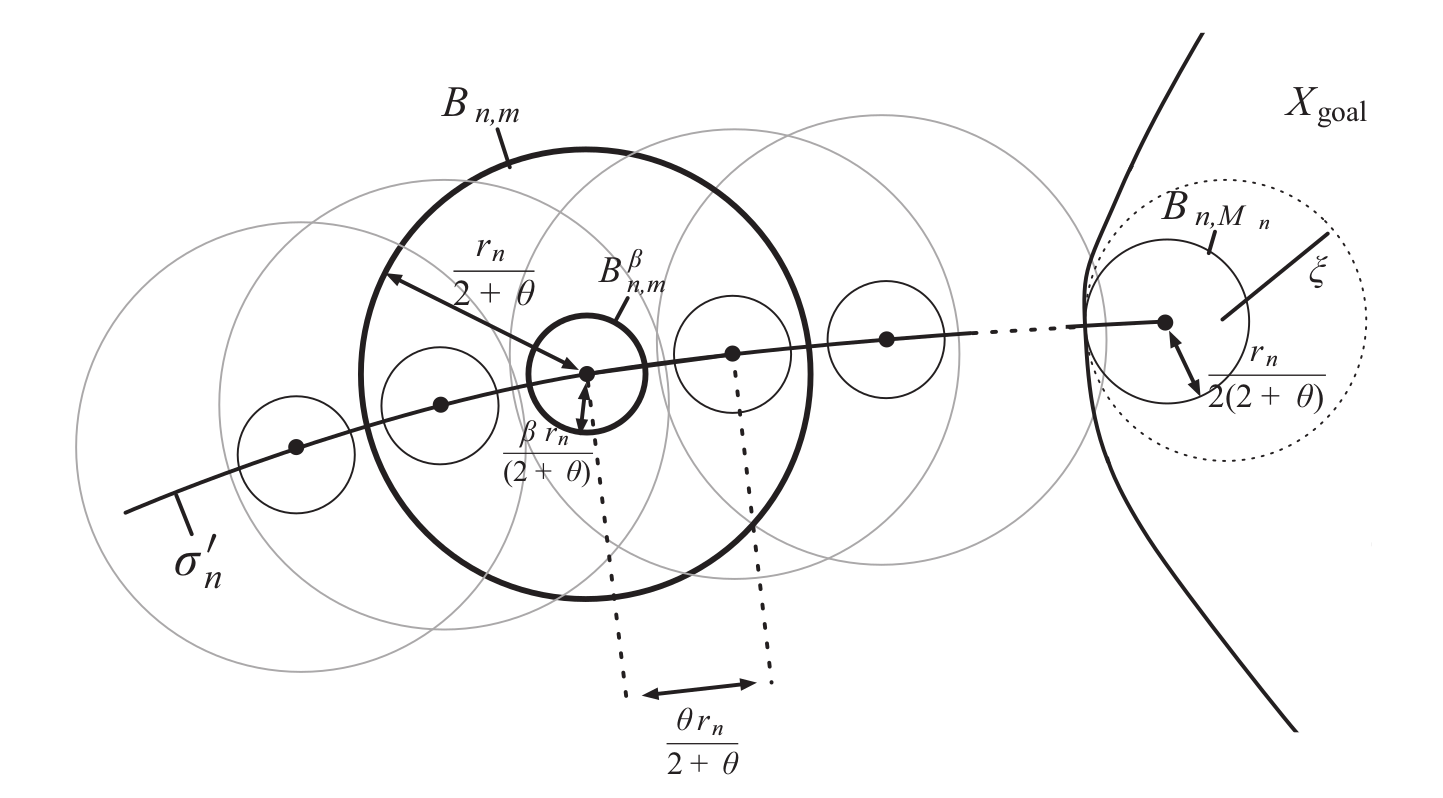
\includegraphics[width=0.7\textwidth]{FMTball.png}
     \caption{FMT ball diagram} 
 \end{figure}
 


\subsection{AO}

TODO <> %TODO
I am not sure I really got around to \textbf{any} of the AO proofs.


\subsection{computational complexity}

\subsubsection{computational complexity}

Generally speaking, one of the biggest bottlenecks is collision checking.

Whatever we can do to minimize the amount of collision checking or speed it up
    will help the most.

Additionally, caching graphs in for instance PRM, as well as intelligently
    determining places to sample, if a path is not found, could be important.

I'm not sure what to say other than that... collision checking seems obvious.

Of course, in my code the nearest neighbor lookups also took a lot of time, but
that is because I implemented it in the simplest way possible.

Perhaps if at some point with large enough dimension, the edge and vertice graph may have
    to be stored in a databse. In this case read and write speeds may become
    important (minimizing calls), or perhaps the wireless connection bandwitch.
    But I don't think this would ever be the bottleneck over collision
    checking.

\section{Numerical Studies}

% TODO numerical
In general, what we care about is determined by real life use cases.
    experimentally confirming the proofs, and charaterizing computational
    complexity. Demonstrating can be used on actual robot.

    E.g. num samples vs (failure rate and pathcost

\subsection{number samples vs path cost, averaged with error bars, ideally for each of the algs  }

TODO: discuss expectations about the graphs for each , and the graphs for algs
compared to each other 

\begin{figure} \centering
    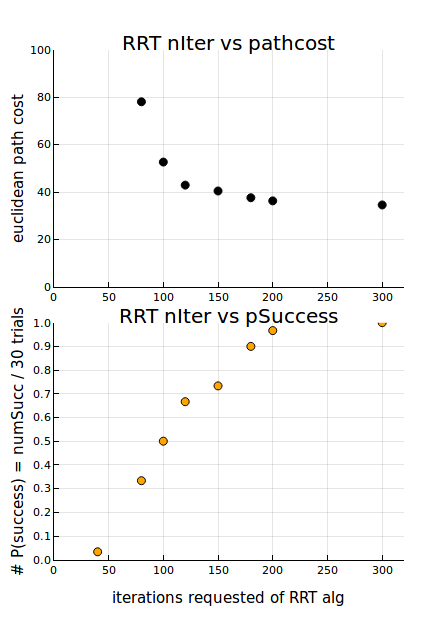
\includegraphics[width=0.5\textwidth]{./RRT_n_pathcost_pSuccess.png}
     \caption{RRT} 
 \end{figure}

\begin{figure} \centering
    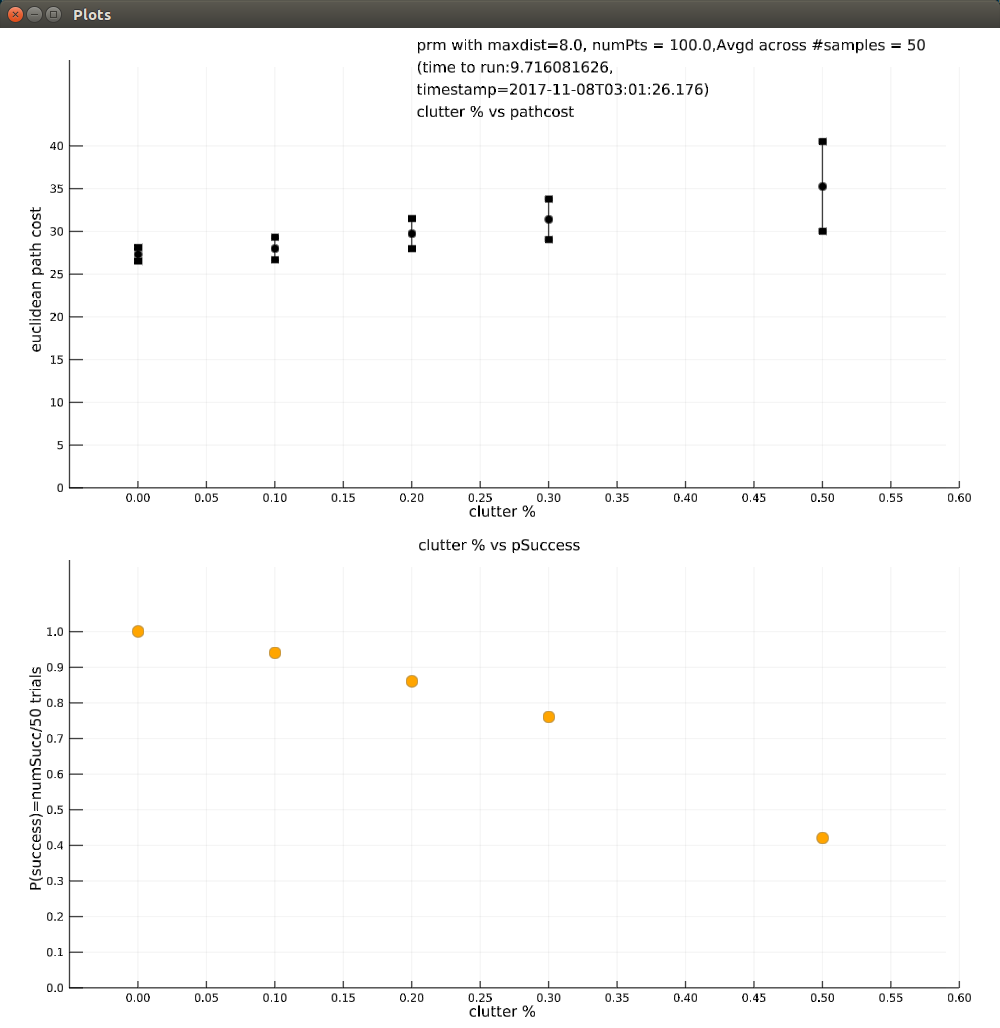
\includegraphics[width=0.5\textwidth]{./PRMn_vs_feasibility_errorbars.png}
     \caption{PRM} 
 \end{figure}

\subsection{ clutter vs pathcost }

\begin{figure} \centering
    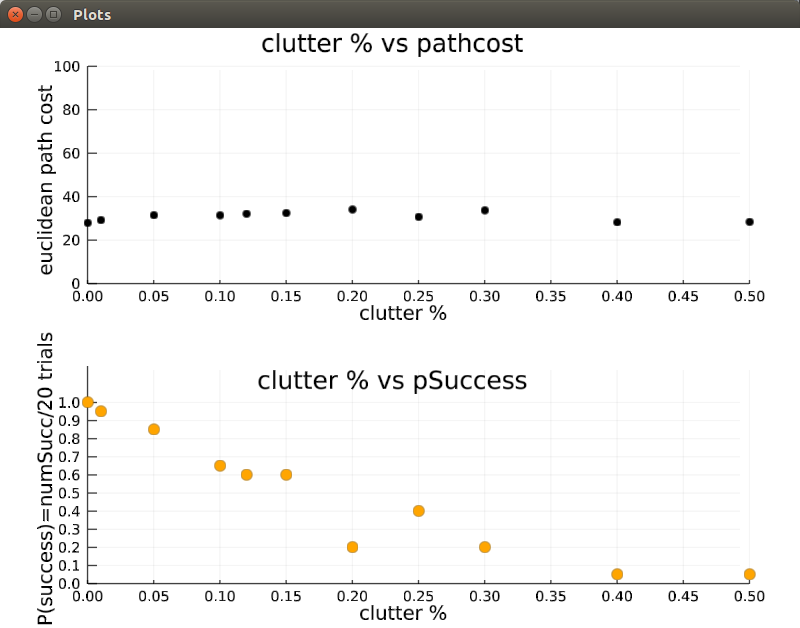
\includegraphics[width=0.5\textwidth]{./PRMcostclutter.png}
     \caption{PRM} 
 \end{figure}


\subsection{  bugtrap }

\begin{figure} \centering
    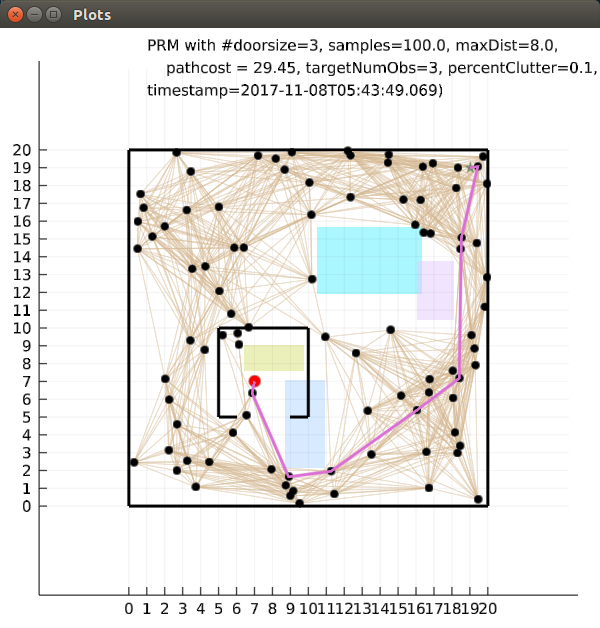
\includegraphics[width=0.5\textwidth]{./PRM_bugtrap_widedoor.png}
     \caption{bugtrap widedoor} 
 \end{figure}

\begin{figure} \centering
    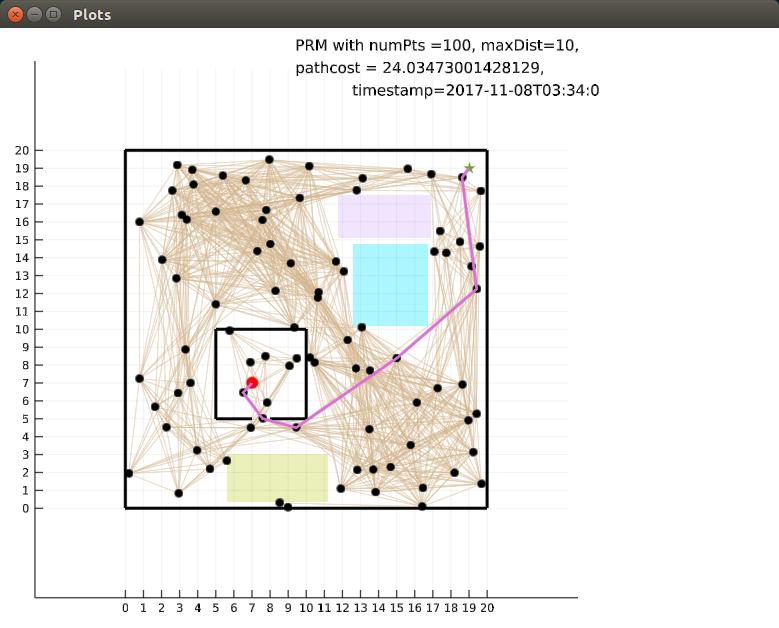
\includegraphics[width=0.5\textwidth]{./PRM_bugtrap.png}
     \caption{some caption} 
 \end{figure}


\begin{figure} \centering
    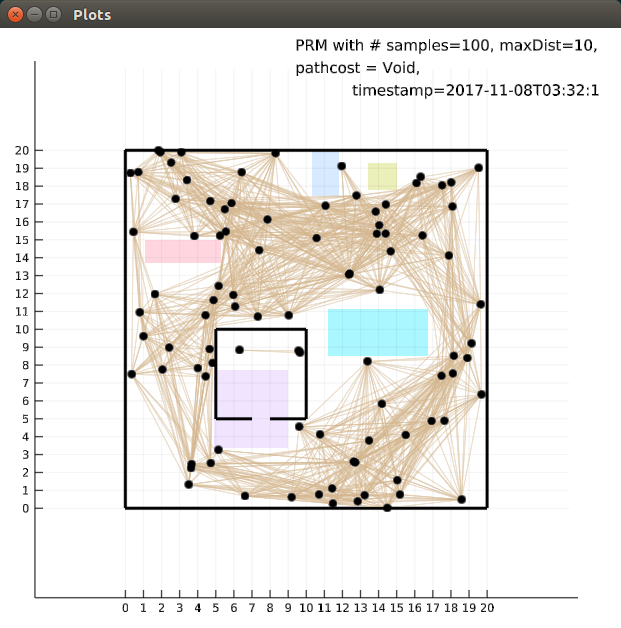
\includegraphics[width=0.5\textwidth]{./PRM_bugtrap_needObsFeasibilityCheck.png}
     \caption{PRM\_bugtrap\_needObsFeasibilityCheck.png} 
 \end{figure}


 
 
 
 
\begin{figure} \centering
    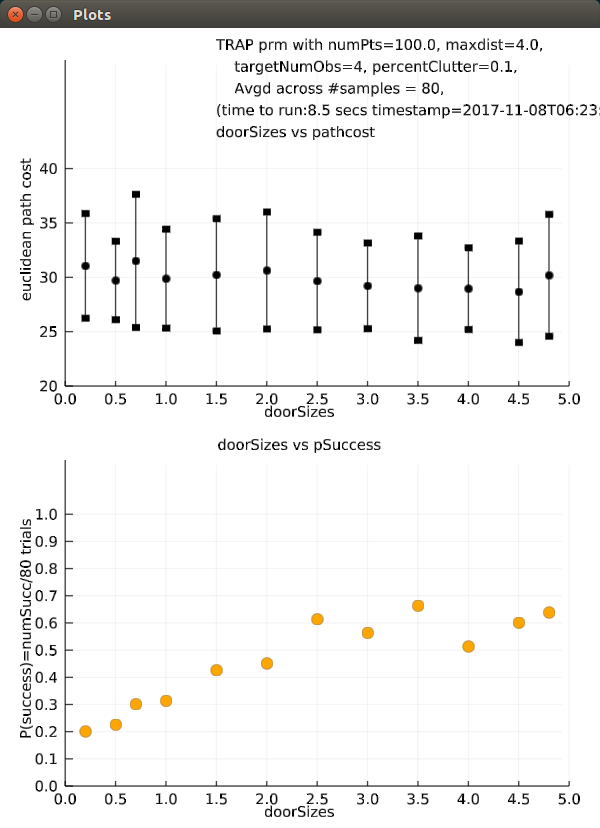
\includegraphics[width=0.5\textwidth]{PRM_bugtrap_doorsize_pSuccess.png}
     \caption{PRM\_bugtrap\PRM\_doorsize\_pSuccess.png} 
 \end{figure}
 
 
 
 
 
    \subsection{Implementation Details}

    Modularity: Roadmap vs Graph Search vs Plotting individual (and possibly
    saving plots of individual runs), vs Plotting and collecting data.

    Walls: collection of lines

    How to deal with graphs so that the information about the actual run (e.g.
    pathcost, connection radius, etc.)
    This probably ate 20-30 hours of Julia frustration... I should have used the
    matplotlib library probably. OR ... just used python. :(
    (e.g. including timestamp very useful).

    Node: should be this or that (include cost in definition, but optionally --
    the optional part ate something like 10 hours in Julia frustration)

    Environment: Apparently spiky obstacles are interesting too. As well as
    higher dimensions.

    Maybe document some Julia things... workflow, types system and common
    errors, where to seek help \footnote{(probably also cover how to atone for your sins of trying weird
    languages not made by large corporations by sacrificing small laptops to the
    programming gods)} And then discuss pros and cons of Julia and warn people about / away from it.

    \subsection{Debugging Protips}

 
 
\begin{figure} \centering
    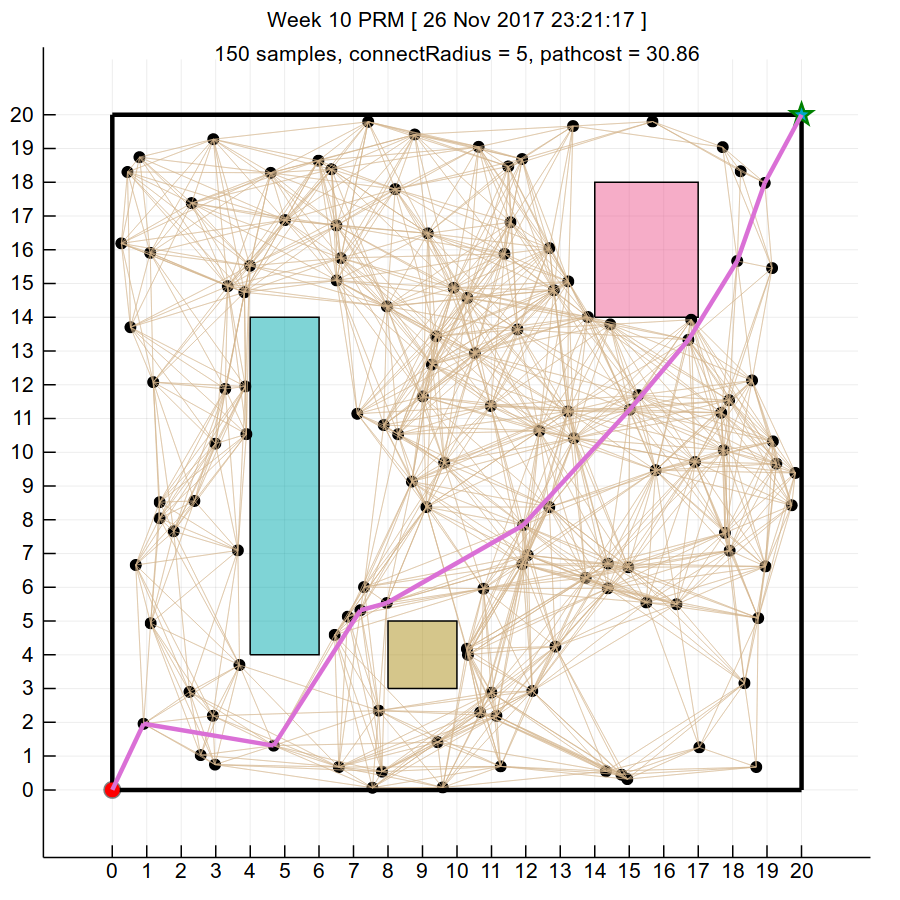
\includegraphics[width=0.5\textwidth]{./PRM_manysamples.png}
     \caption{prm many samples}
 \end{figure}


    Trees should not be graphs (no cyclic components)

    \\

    Lines should not cross obstacles

    \\

    Plot n = 500 points etc. to see how it covers the room


\section{Results}

    \subsection{num samples vs (failure rate and pathcost)}
    \subsubsection{PRM}

    todo RRT, RRT*, PRM* double check this

    \subsection{\%clutter vs (pathcost and feasibility)}



%%%%%%%%%%%%%%%%%%%%%%%%%%%%%%%

\section{Things I learned}

I learned about reading math papers. 99\% of the symbols are defined in the
paper, you just have to be patient about finding the defintion either earlier or later in
the paper, or perhaps in the appendix somewhere. 

    Reading a page of proofs takes >10 hours a page. Should learn to pick
    battles (understanding some of the stuff may not be critical to
    understanding the approach of the proof, and also some time should be spent
    on what the proof tells us / how the proof is useful)

    Abstractions -- for instance, we don't need to define a robot size or
    clearance needed, we can
    simply "increase" the size of the obstacles

<The set minus, the gets, the union and and signs, supremeum and infinimum, >

%% explain those 

I also learned about the differences between sampling-based motion planning and
nonlinear convex optimazation approaches, and which one is more suited than the
other.

Latex is pretty reasonable, I had some horrific first experience and avoided it
    since. But just installed all 3 GB of packages or whatever (via sudo apt
    install texmaker) and previewed templates on sharelatex and now all set.

I also learned a bit about keeping in mind the overall goal vs. getting stuck on
any particular milestone / to-do item. I don't think I had the chance to do so,
but I wish I had been able to make more executive decisions about what to
accomplish. 

\section{Reflection}

This rotation was very enjoyable, I've never worked through a proof before. I
feel less intimidated by algorithmic notation and proofs now that I have a
better idea what they are. In that sense, forcing myself to work through this
rotation helped me out a lot. I also hadn't thought math was fun since middle
school, so it was really nice to hang out with math majors who were really
enthusiastic about math. Hopefully this feeling will keep me going when I take
math courses and have to do graded things.

My choice of Julia was a tad unfortunate, although it was kind of neat to see.
In retrospect, I really didn't want to deal with MATLAB (which was glitchy on
linux, and I didn't have a windows install at the time. I miss public
computers), and I thought it might be annoying to understand what was going on
with numpy. But in the end I used no matrices... so... python was a much better
way to go. I didn't think to ask graph python people (instead of robotics
people) to show me a workflow,
though a friend helped with the computer vision homework and I got to know the
python syntax a lot better.

An example of why Julia documentation and I did not get along:
https://github.com/scheinerman/Permutations.jl

I think to some extent I expected it to be a little rough to pick to do a PhD in a new-ish
field, and then to take both computer vision (linear algebra) and this rotation
(statistics) when I hadn't taken a math class in a while. But it was even
rougher than I imagined...

Regardless I certainly learned a lot compared to the beginning of the semester!
I'm happy, this is part of why I decided to go to grad school. It was
neat to see it all tying together, AI and this rotation and even some of the
ideas from computer vision.

In the future, I intend to take more math classes and programming classes. I
also intend to not use Julia again for a long while. After I switched from
MATLAB to python for computer vision final project, it was amazing, I'd
forgotten that programming could actually be pleasant and fun, and I imagine
something similar will happen with switching from Julia to Python.

\section{Conclusion}

Math is so cool!

\section{Thanks}

People who have helped me understand math / Julia:

\begin{itemize}
    \item Irina Tolkova
    \item Eric Lu 
    \item Ambarish Chattopadhyay
    \item Robin Deits
    \item Misc. patient strangers online who dealt with my deep incoherent
        frustration... I will look their names up later 
\end{itemize}

Thanks to my advisor Lucas Janson for sparing an hour a week to patiently trying
to explain things to me in a way that made sense to me, for writing
numerous recommmendation letters, dealing with my continual work tardiness, and
helping me figure out what I want to do in terms of research.

%%%%%%%%%%%%%%%%%%%%%%%%%%%%%%%%

\section{References}

\begin{thebibliography}{1}

\bibitem{PRM} 
        LaValle, S. M. (1998). Rapidly-exploring random trees: A new tool for
        path planning.
        \href{http://bloom.personalrobotics.ri.cmu.edu/files/courses/papers/Kavraki98-prm.pdf}{Paper link} 

\bibitem{RRT*} 
        Karaman, S., & Frazzoli, E. (2011). Sampling-based algorithms for
        optimal motion planning. The international journal of robotics research,
        30(7), 846-894.
        \href{https://arxiv.org/pdf/1105.1186}{PDF link}


\bibitem{FMT*} Fast Marching Tree {\em Imperial Japan 1800-1945} 2015.
    Janson, L., Schmerling, E., Clark, A., & Pavone, M. (2015). Fast marching
        tree: A fast marching sampling-based method for optimal motion planning
        in many dimensions. The International journal of robotics research,
        34(7), 883-921.
        \href{http://journals.sagepub.com/doi/10.1177/0278364915577958}{Article
        DOI link} 
        \href{ https://arxiv.org/pdf/1306.3532.pdf}{PDF link}


\end{thebibliography}


%%%%%%%%%%%%%%%%%%%%%%%%%%%%%%%%%
%http://cs229.stanford.edu/notes/cs229-notes10.pdf (PCA)


%PCA (Andrew Ng) https://www.youtube.com/watch?v=T-B8muDvzu0&index=83&list=PLLssT5z_DsK-h9vYZkQkYNWcItqhlRJLN


%https://link-springer-com.ezp-prod1.hul.harvard.edu/book/10.1007%2F978-0-387-87811-9#about
\end{document}

